\documentclass[border=10pt]{standalone}
\usepackage{pgfplots}
\pgfplotsset{compat=1.18}
\usepackage{amsmath}
 
\begin{document}
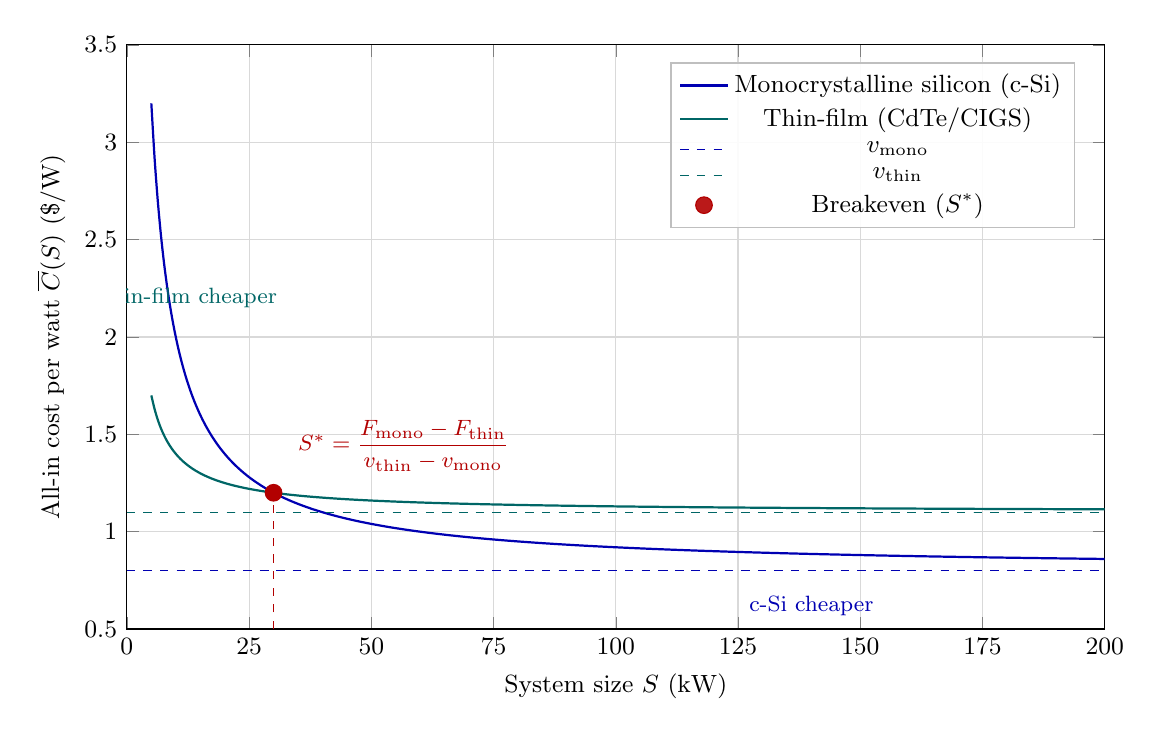
\begin{tikzpicture}
\begin{axis}[
    width=14cm,
    height=9cm,
    xlabel={System size $S$ (kW)},
    ylabel={All-in cost per watt $\overline{C}(S)$ (\$/W)},
    xmin=0, xmax=200,
    ymin=0.5, ymax=3.5,
    domain=5:200,
    samples=300,
    grid=both,
    grid style={line width=0.2pt, draw=gray!20},
    major grid style={line width=0.4pt, draw=gray!30},
    legend style={
        at={(0.97,0.97)},
        anchor=north east,
        font=\small,
        draw=gray!50,
        fill=white,
        fill opacity=0.9,
        text opacity=1,
    },
    tick label style={font=\small},
    label style={font=\small},
    scaled x ticks=false,
    y tick label style={/pgf/number format/fixed, /pgf/number format/precision=2},
    xtick={0,25,50,75,100,125,150,175,200},
    ytick={0.50,1.00,1.50,2.00,2.50,3.00,3.50},
    clip=true,
]
 
% ---------------------------------------------------------------
%  Consumer model: C_bar(S) = F / S + v
%
%  S  = system size (kW)
%  F  = fixed project costs ($k * kW units so F/S -> $/W)
%  v  = variable all-in cost per watt
%
%  c-Si:      high F (premium modules require precise engineering,
%             optimized mounting for heavier panels)
%             low v  (high W/m^2 efficiency -> less area-driven
%             BOS per watt at the margin)
%  Thin-film: low F  (simple installation, lightweight modules)
%             high v (low efficiency -> area-proportional BOS
%             costs per watt accumulate with system size)
%
%  Parameters (illustrative):
%    c-Si:      F_mono = 12,  v_mono = 0.80 ($/W)
%    Thin-film: F_thin = 3,   v_thin = 1.10 ($/W)
%
%  Breakeven:  S* = (F_mono - F_thin) / (v_thin - v_mono)
%                 = 9 / 0.30 = 30 kW
% ---------------------------------------------------------------
 
% --- c-Si curve ---
\addplot[
    blue!70!black,
    thick,
    smooth,
] {12/x + 0.80};
\addlegendentry{Monocrystalline silicon (c-Si)}
 
% --- Thin-film curve ---
\addplot[
    teal!80!black,
    thick,
    smooth,
] {3/x + 1.10};
\addlegendentry{Thin-film (CdTe/CIGS)}
 
% --- Asymptotes (variable-cost floors) ---
\addplot[
    blue!70!black,
    dashed,
    thin,
    domain=0:200,
] {0.80};
\addlegendentry{$v_{\mathrm{mono}}$}
 
\addplot[
    teal!80!black,
    dashed,
    thin,
    domain=0:200,
] {1.10};
\addlegendentry{$v_{\mathrm{thin}}$}
 
% --- Breakeven point ---
\addplot[
    only marks,
    mark=*,
    mark size=3pt,
    red!70!black,
] coordinates {(30, 1.20)};
\addlegendentry{Breakeven ($S^{*}$)}
 
% --- Vertical dashed line at breakeven ---
\draw[red!70!black, dashed, thin]
    (axis cs:30, 0.5) -- (axis cs:30, 1.20);
 
% --- Annotation ---
\node[
    anchor=south west,
    font=\footnotesize,
    red!70!black,
    align=left,
] at (axis cs:33, 1.26) {%
    $S^{*} = \dfrac{F_{\mathrm{mono}} - F_{\mathrm{thin}}}{v_{\mathrm{thin}} - v_{\mathrm{mono}}}$%
};
 
% --- Region labels ---
\node[
    font=\footnotesize,
    teal!80!black,
    align=center,
] at (axis cs:12, 2.2) {Thin-film cheaper};
 
\node[
    font=\footnotesize,
    blue!70!black,
    align=center,
] at (axis cs:140, 0.62) {c-Si cheaper};
 
\end{axis}
\end{tikzpicture}
\end{document}